\chapter{Psalm 18}

\begin{figure}
  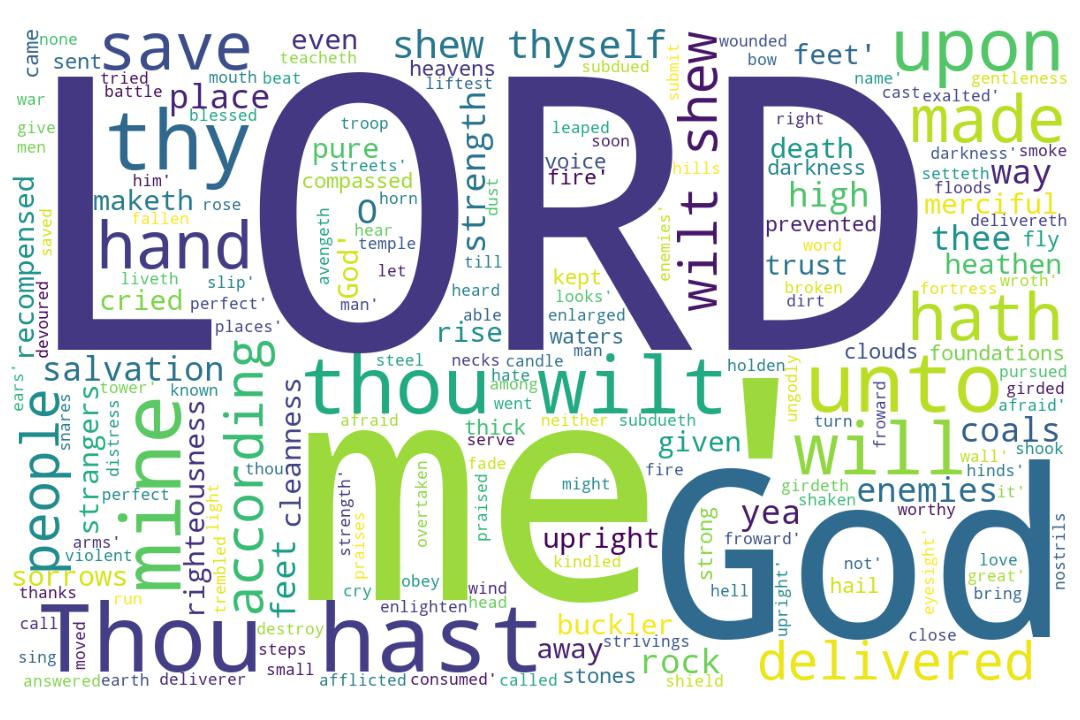
\includegraphics[width=\linewidth]{19OT-Psalms/Psalm18-WordCloud.jpg}
  \caption{Psalm 18 Word Cloud}
  \label{fig:Psalm 18 word Cloud}
\end{figure}

\marginpar{\scriptsize \centering \fcolorbox{bone}{lime}{\textbf{MY SOURCE}}\\ (Psalm 18:1--50) \begin{compactenum}[I.][8]
	\item My Source of \textbf{Strength} \index[scripture]{Psalms!Psa 018:01}(Psalm 18:1, \index[scripture]{Psalms!Psa 018:32}Psa 18:32, \index[scripture]{Psalms!Psa 018:39}Psalm 18:39)
	\item My Source of \textbf{Salvation} \index[scripture]{Psalms!Psa 018:02}(Psa 18:2)
	\item My Source of \textbf{Solace} \index[scripture]{Psalms!Psa 018:06}(Psa 18:6)
	\item My Source of \textbf{Security} \index[scripture]{Psalms!Psa 018:18}(Psa 18:18)
	\item My Source of \textbf{Sympathy} \index[scripture]{Psalms!Psa 018:25}(Psa 18:25)
	\item My Source of \textbf{Skill} \index[scripture]{Psalms!Psa 018:34}(Psa 18:34)
	\item My Source of \textbf{Song} \index[scripture]{Psalms!Psa 018:49}(Psa 18:49)
\end{compactenum}}

\marginpar{\scriptsize \centering \fcolorbox{bone}{yellow}{\textbf{A MAN OF WAR}}\\ (Psalm 18:1--50)\begin{compactenum}[I.][8]
	\item The Lord is a \textbf{Fortress} \index[scripture]{Psalms!Psa 018:02}(Psa 18:2)
	\item The Lord is a \textbf{Deliverer} \index[scripture]{Psalms!Psa 018:02}(Psa 18:2)
	\item The Lord is my \textbf{Strength} \index[scripture]{Psalms!Psa 018:02}(Psa 18:2)
	\item The Lord is a \textbf{Buckler} \index[scripture]{Psalms!Psa 018:02}(Psa 18:2)
	\item The Lord is a \textbf{High Tower} \index[scripture]{Psalms!Psa 018:02}(Psa 18:2)
	\item The Lord is a \textbf{Horn} \index[scripture]{Psalms!Psa 018:02}(Psa 18:2)
	\item The Lord is a \textbf{Rock} \index[scripture]{Numbers!Num 018:02}\index[scripture]{2 Chronicles!2Chr 13:14}\index[scripture]{Psalms!Psa 018:02}(Num 10:2, 2Chr 13:14, Psa 18:2)
\end{compactenum}}

\footnote{\textcolor[cmyk]{0.99998,1,0,0}{\hyperlink{TOC}{Return to end of Table of Contents.}}}\footnote{\href{https://www.audioverse.org/english/audiobibles/books/ENGKJV/O/Ps/1}{\textcolor[cmyk]{0.99998,1,0,0}{Psalms Audio}}}\textcolor[cmyk]{0.99998,1,0,0}{To the chief Musician, \emph{A Psalm} of David, the servant of the LORD, who spake unto the LORD the words of this song in the day \emph{that} the LORD delivered him from the hand of all his enemies, and from the hand of Saul: And he said,}\\
\\
\textcolor[cmyk]{0.99998,1,0,0}{I will love thee, O LORD, \fcolorbox{bone}{lime}{my strength}.}
[2] \textcolor[cmyk]{0.99998,1,0,0}{The LORD \emph{is} my rock, and my fortress, and my deliverer; my God, my strength, in whom I will trust; my buckler, and the \fcolorbox{bone}{lime}{horn of my salvation}, \emph{and} my high tower.}
[3] \textcolor[cmyk]{0.99998,1,0,0}{I will call upon the LORD, \emph{who} \emph{is} \emph{worthy} \fcolorbox{bone}{bone}{to} be praised: so shall I be saved from mine enemies.}
[4] \textcolor[cmyk]{0.99998,1,0,0}{The sorrows of death compassed me, and the floods of ungodly men made me afraid.}
[5] \textcolor[cmyk]{0.99998,1,0,0}{The sorrows of hell compassed me about: the snares of death prevented me.}
[6] \textcolor[cmyk]{0.99998,1,0,0}{In my distress I \fcolorbox{bone}{lime}{called upon the LORD}, and cried unto my God: he heard my voice out of his temple, and my cry came before him, \emph{even} into his ears.}
[7] \textcolor[cmyk]{0.99998,1,0,0}{Then the earth shook and trembled; the foundations also of the hills moved and were shaken, because he was wroth.}
[8] \textcolor[cmyk]{0.99998,1,0,0}{There went up a smoke out of his nostrils, and fire out of his mouth devoured: coals were kindled by it.}
[9] \textcolor[cmyk]{0.99998,1,0,0}{He bowed the heavens also, and came down: and darkness \emph{was} under his feet.}
[10] \textcolor[cmyk]{0.99998,1,0,0}{And he rode upon a cherub, and did fly: yea, he did fly upon the wings of the wind.}
[11] \textcolor[cmyk]{0.99998,1,0,0}{He made darkness his secret place; his pavilion round about him \emph{were} dark waters \emph{and} thick clouds of the skies.}
[12] \textcolor[cmyk]{0.99998,1,0,0}{At the brightness \emph{that} \emph{was} before him his thick clouds passed, hail \emph{stones} and coals of fire.}
[13] \textcolor[cmyk]{0.99998,1,0,0}{The LORD also thundered in the heavens, and the Highest gave his voice; hail \emph{stones} and coals of fire.}\footnote{\textbf{1 Samuel 7:1} - And as Samuel was offering up the burnt offering, the Philistines drew near to battle against Israel: but the LORD thundered with a great thunder on that day upon the Philistines, and discomfited them; and they were smitten before Israel.}\footnote{\textbf{2 Samuel 22:14} -  The LORD thundered from heaven, and the most High uttered his voice.}\footnote{\textbf{John 12:29} - The people therefore, that stood by, and heard it, said that it thundered: others said, An angel spake to him.}
[14] \textcolor[cmyk]{0.99998,1,0,0}{Yea, he sent out his arrows, and scattered them; and he shot out lightnings, and discomfited them.}
[15] \textcolor[cmyk]{0.99998,1,0,0}{Then the channels of waters were seen, and the foundations of the world were discovered at thy rebuke, O LORD, at the blast of the breath of thy nostrils.}
[16] \textcolor[cmyk]{0.99998,1,0,0}{He sent from above, he took me, he drew me out of many waters.}
[17] \textcolor[cmyk]{0.99998,1,0,0}{He delivered me from my strong enemy, and from them which hated me: for they were too strong for me.}
[18] \textcolor[cmyk]{0.99998,1,0,0}{They prevented me in the day of my calamity: but \fcolorbox{bone}{lime}{the LORD was my stay}.}
[19] \textcolor[cmyk]{0.99998,1,0,0}{He brought me forth also into a large place; he delivered me, because he delighted in me.}\footnote{\textbf{2 Samuel 22:20} - He brought me forth also into a large place: he delivered me, because he delighted in me.}\footnote{\textbf{Psalm 118:5} - I called upon the LORD in distress: the LORD answered me, and set me in a large place.}\footnote{\textbf{Hosea 4:16} - For Israel slideth back as a backsliding heifer: now the LORD will feed them as a lamb in a large place.}
[20] \textcolor[cmyk]{0.99998,1,0,0}{The LORD rewarded me according \fcolorbox{bone}{bone}{to} my righteousness; according \fcolorbox{bone}{bone}{to} the cleanness of my hands hath he recompensed me.}
[21] \textcolor[cmyk]{0.99998,1,0,0}{For I have kept the ways of the LORD, and have not wickedly departed from my God.}
[22] \textcolor[cmyk]{0.99998,1,0,0}{For all his judgments \emph{were} before me, and I did not put away his statutes from me.}
[23] \textcolor[cmyk]{0.99998,1,0,0}{I was also upright before him, and I kept myself from mine iniquity.}
[24] \textcolor[cmyk]{0.99998,1,0,0}{Therefore hath the LORD recompensed me according \fcolorbox{bone}{bone}{to} my righteousness, according \fcolorbox{bone}{bone}{to} the cleanness of my hands in his eyesight.}
[25] \textcolor[cmyk]{0.99998,1,0,0}{With the merciful thou wilt \fcolorbox{bone}{lime}{shew thyself merciful}; with an upright man thou wilt shew thyself upright;}
[26] \textcolor[cmyk]{0.99998,1,0,0}{With the pure thou wilt shew thyself pure; and with the froward thou wilt shew thyself froward.}
[27] \textcolor[cmyk]{0.99998,1,0,0}{For thou wilt save the afflicted people; but wilt bring down high looks.}
[28] \textcolor[cmyk]{0.99998,1,0,0}{For thou wilt light my candle: the LORD my God will enlighten my darkness.}
[29] \textcolor[cmyk]{0.99998,1,0,0}{For by thee I have run through a troop; and by my God have I leaped over a wall.}
[30] \textcolor[cmyk]{0.99998,1,0,0}{\emph{As} \emph{for} God, his way \emph{is} perfect: the word of the LORD is tried: he \emph{is} a buckler \fcolorbox{bone}{bone}{to} all those that trust in him.}\footnote{\textbf{Psalm 12:6} - The words of the LORD are pure words: as silver tried in a furnace of earth, purified seven times.}  
[31] \textcolor[cmyk]{0.99998,1,0,0}{For who \emph{is} God save the LORD? or who \emph{is} a rock save our God?}
[32] \textcolor[cmyk]{0.99998,1,0,0}{\emph{It} \emph{is} God that girdeth me with strength, and maketh my way perfect.}
[33] \textcolor[cmyk]{0.99998,1,0,0}{He maketh my feet like hinds' \emph{feet}, and setteth me upon my high places.}
[34] \textcolor[cmyk]{0.99998,1,0,0}{He \fcolorbox{bone}{lime}{teacheth my hands} \fcolorbox{bone}{bone}{to} war, so that a bow of steel is broken by mine arms.}
[35] \textcolor[cmyk]{0.99998,1,0,0}{Thou hast also given me the shield of thy salvation: and thy right hand hath holden me up, and thy gentleness hath made me great.}
[36] \textcolor[cmyk]{0.99998,1,0,0}{Thou hast enlarged my steps under me, that my feet did not slip.}
[37] \textcolor[cmyk]{0.99998,1,0,0}{I have pursued mine enemies, and overtaken them: neither did I turn again till they were consumed.}
[38] \textcolor[cmyk]{0.99998,1,0,0}{I have wounded them that they were not able \fcolorbox{bone}{bone}{to} rise: they are fallen under my feet.}
[39] \textcolor[cmyk]{0.99998,1,0,0}{For thou hast girded me with strength unto the battle: thou hast subdued under me those that rose up against me.}
[40] \textcolor[cmyk]{0.99998,1,0,0}{Thou hast also given me the necks of mine enemies; that I might destroy them that hate me.}
[41] \textcolor[cmyk]{0.99998,1,0,0}{They cried, but \emph{there} \emph{was} none \fcolorbox{bone}{bone}{to} save \emph{them:} \emph{even} unto the LORD, but he answered them not.}
[42] \textcolor[cmyk]{0.99998,1,0,0}{Then did I beat them small as the dust before the wind: I did cast them out as the dirt in the streets.}
[43] \textcolor[cmyk]{0.99998,1,0,0}{Thou hast delivered me from the strivings of the people; \emph{and} thou hast made me the head of the heathen: a people \emph{whom} I have not known shall serve me.}
[44] \textcolor[cmyk]{0.99998,1,0,0}{As soon as they hear of me, they shall obey me: the strangers shall submit themselves unto me.}
[45] \textcolor[cmyk]{0.99998,1,0,0}{The strangers shall fade away, and be afraid out of their close places.}
[46] \textcolor[cmyk]{0.99998,1,0,0}{The LORD liveth; and blessed \emph{be} my rock; and let the God of my salvation be exalted.}
[47] \textcolor[cmyk]{0.99998,1,0,0}{\emph{It} \emph{is} God that avengeth me, and subdueth the people under me.}
[48] \textcolor[cmyk]{0.99998,1,0,0}{He delivereth me from mine enemies: yea, thou liftest me up above those that rise up against me: thou hast delivered me from the violent man.}
[49] \textcolor[cmyk]{0.99998,1,0,0}{Therefore will I give thanks unto thee, O LORD, among the heathen, and \fcolorbox{bone}{lime}{sing praises} unto thy name.}
[50] \textcolor[cmyk]{0.99998,1,0,0}{Great deliverance giveth he \fcolorbox{bone}{bone}{to} his king; and sheweth mercy \fcolorbox{bone}{bone}{to} his anointed, \fcolorbox{bone}{bone}{to} David, and \fcolorbox{bone}{bone}{to} his seed for evermore.}





